\documentclass[10pt]{beamer}

\usetheme[progressbar=frametitle]{metropolis}
\usepackage{appendixnumberbeamer}

\usepackage{booktabs}
\usepackage[scale=2]{ccicons}

\usepackage{pgfplots}
\usepgfplotslibrary{dateplot}

\usepackage{xspace}
\newcommand{\themename}{\textbf{\textsc{metropolis}}\xspace}

\title{Introduction to AI & ML}
\subtitle{EE1390}
% \date{\today}
\date{}
\author{Pragati Modi : EE17BTECH11029 \\ Nishma N : EE17BTECH11025 }
\institute{IIT HYDERABAD}
% \titlegraphic{\hfill\includegraphics[height=1.5cm]{logo.pdf}}

\begin{document}

\maketitle

\begin{frame}[fragile]{Problem}
Find the equation of the tangent to the circle at the point \\
\begin{pmatrix} 1 \\ -1 \end{pmatrix}\\
whose center is the point of intersection of the straight lines \\
\begin{equation*}
\begin{pmatrix} 2 \ 1 \end{pmatrix}x = 3\\
\end{equation*}
\begin{equation*}
\begin{pmatrix} 1 \ -1 \end{pmatrix}x = 1\\
\end{equation*}
\end{frame}

\begin{frame}{Solution}
Let O be the center of the circle C given by the intersection of the straight lines \\
\begin{equation*}
\begin{pmatrix} 2 \ 1 \end{pmatrix}x = 3
\end{equation*}
\begin{equation*}
\begin{pmatrix} 1 \ -1 \end{pmatrix}x = 1\\
\end{equation*}
\end{frame}

{
\begin{frame}
The intersection point of two lines given by \\
\[ n_{1}^{T}x = p_{1}\] \\ \[ n_{2}^{T}x = p_{2} \] can be given by \\
\begin{equation*}
\begin{split}
    \begin{pmatrix}
    n_{1}^{T} \\
    n_{2}^{T}
    \end{pmatrix}
    x = 
    \begin{pmatrix}
    p_{1} \\
    p_{2}
    \end{pmatrix}
\end{split}
\end{equation*}
let
\begin{equation*}
\begin{split}
     N^{T} = 
    \begin{pmatrix}
    n_{1}^{T} \\
    n_{2}^{T}
    \end{pmatrix}
    and\ p =
    \begin{pmatrix}
    p_{1} \\
    p_{2}
    \end{pmatrix}
\end{split}
\end{equation*}
\end{frame}
}

{
\begin{frame}
Thus,
\begin{equation*}
\begin{split}
     N^{T}x &= p \\
    N &= 
    \begin{pmatrix}
    n_{1} \
    n_{2}
    \end{pmatrix} \\
    x &= N^{-T}p \\
\end{split}
\end{equation*}
Since O is the point of intersection 
\begin{equation*}
\begin{split}
O &= 
\begin{pmatrix}
\frac{1}{3} \ \frac{1}{3} \\
\frac{1}{3} \ \frac{-2}{3} \\
\end{pmatrix}
\begin{pmatrix}
3 \\ 1
\end{pmatrix} \\
O &= \begin{pmatrix}
\frac{4}{3} \\
\frac{1}{3}
\end{pmatrix}   
\end{split}
\end{equation*}
\end{frame}
}

\begin{frame}
\begin{equation*}
\begin{split}
    Let\ k &= 
    \begin{pmatrix}
    0 \ 1 \\
    -1 \ 0 
    \end{pmatrix}\\
    t &=  k*OA\\
    &= \begin{pmatrix}
    \frac{4}{3} \\ \frac{-1}{3}
    \end{pmatrix} \\
    Q &= t^{T} \\
    &= \begin{pmatrix}
    \frac{4}{3} \ \frac{-1}{3}
    \end{pmatrix}
\end{split}
\end{equation*}

\end{frame}

\begin{frame}
Equation of the tangent
\begin{equation*}
\begin{split}
    Qx = constant
\end{split} \\
\end{equation*}
   A is the point 
  \begin{pmatrix}
  1 \\ -1
  \end{pmatrix} \\
  Since x = A satisfies the above equation \\
  We get
\begin{equation*}
    \begin{pmatrix}
    4 \ -1
    \end{pmatrix}
    x = 5
\end{equation*}
which is the equation of the tangent to the circle C at the point \begin{pmatrix}
1 \\ -1
\end{pmatrix}
\end{frame}

\begin{frame}
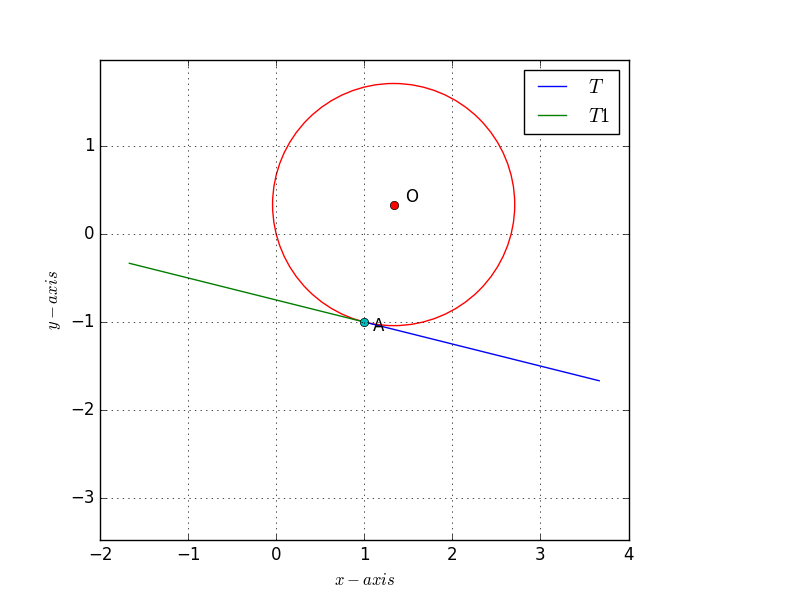
\includegraphics[scale=0.6]{figure.png}
\end{frame}
    
\end{frame}
\end{frame}

\end{document}
